\documentclass[11pt]{article}

% ---------- packages ----------
\usepackage[utf8]{inputenc}
\usepackage[T1]{fontenc}
\usepackage{lmodern}
\usepackage[a4paper,margin=1in]{geometry}
\usepackage{amsmath,amssymb}
\usepackage{bm}
\usepackage{booktabs}
\usepackage{tabularx}
\usepackage{array}
\usepackage{microtype}
\usepackage{enumitem}
\usepackage{xcolor}
\usepackage{titlesec}
\usepackage{tikz}
\usetikzlibrary{positioning,arrows.meta,calc,patterns,fit,backgrounds}
\usepackage{float}
\usepackage{caption}
\usepackage{listings}
\usepackage[hidelinks,colorlinks=true,linkcolor=teal!60!black,citecolor=teal!60!black,urlcolor=teal!60!black]{hyperref}

% ---------- styling ----------
\definecolor{accent}{RGB}{20,90,90}
\definecolor{accent2}{RGB}{180,95,30}
\definecolor{boxbg}{RGB}{245,247,247}
\titleformat{\section}{\large\bfseries\color{accent}}{\thesection}{0.6em}{}
\titleformat{\subsection}{\normalsize\bfseries}{\thesubsection}{0.6em}{}
\setlist{itemsep=2pt,topsep=3pt,parsep=0pt}
\renewcommand{\arraystretch}{1.25}
\newcolumntype{Y}{>{\raggedright\arraybackslash}X}

% ---------- algorithm float + listings pseudocode ----------
\newfloat{algorithm}{tbp}{loa}
\floatname{algorithm}{Algorithm}
\lstdefinestyle{pseudo}{
  basicstyle=\ttfamily\small,
  keywordstyle=\color{accent}\bfseries,
  keywordstyle=[2]\color{accent2}\bfseries,
  commentstyle=\itshape\color{gray},
  morekeywords={for,each,if,else,then,return,while,do,end,Input,Output,Require,Ensure},
  morekeywords=[2]{CoarseStep,Restrict,Prolong,Blend,Predict,Project,Exchange,Schwarz},
  columns=fullflexible,
  keepspaces=true,
  mathescape=false,
  showstringspaces=false,
  frame=none,
  xleftmargin=1.2em,
  aboveskip=2pt,belowskip=2pt,
}

% ---------- math shortcuts ----------
\newcommand{\R}{\mathbb{R}}
\newcommand{\Rop}{\mathcal{R}}
\newcommand{\Eop}{\mathcal{E}}
\newcommand{\Gfine}{\mathcal{G}_{\Phi}}
\newcommand{\Gcoarse}{\bar{\mathcal{G}}_{\Psi}}
\newcommand{\F}{\mathcal{F}}
\newcommand{\half}{\tfrac{1}{2}}

\title{\vspace{-1.2cm}\textbf{Recommended Approach: A Domain-Decomposed Neural Surrogate}\\[2pt]
\large Detailed end-to-end design --- companion to the survey note}
\author{Research note --- \texttt{pyurbanair} / domain-decomposition surrogates}
\date{\today}

\begin{document}
\maketitle
\vspace{-0.5cm}

\noindent
This companion expands the recommendation from the survey into an implementable
design. Section~\ref{sec:notation} fixes notation. Section~\ref{sec:recA} gives
the primary recommendation in full --- formulas, figures, and pseudo-code.
Section~\ref{sec:recB} gives a leaner alternative with stronger consistency
guarantees. Section~\ref{sec:choice} compares them, and
Section~\ref{sec:mapping} maps both onto the existing codebase. Citations refer
to the shared bibliography \texttt{references.bib}.

\section{Scope and notation}\label{sec:notation}

Write the discretized state on the full grid as
$\bm S_t \in \R^{C\times N_z\times N_y\times N_x}$, with $C$ channels (the
velocity components $u,v,w$ and pressure $p$), a static geometry mask
$\bm m \in \{0,1\}^{N_z\times N_y\times N_x}$ ($1$ = fluid), and an inflow
parameter vector $\bm p_t$. The reference LES solver advances the state by one
output step,
\begin{equation}
\bm S_{t+1} = \F(\bm S_t,\, \bm p_t,\, \bm m),
\label{eq:truth}
\end{equation}
and the surrogate's job is to learn a cheap approximation of $\F$. The current
\texttt{pyurbanair} surrogate is a single translation-equivariant convolutional
map $\Gfine(\bm S_t, \bm p_t, \bm m)\approx \bm S_{t+1}$ applied to the whole
grid; the goal is to replace the whole-grid application by a tiling of a shared
network over subdomains.

\paragraph{Subdomains, halos, restriction.}
Cover the grid by $M$ overlapping subdomains $\{\Omega_i\}_{i=1}^M$. Each has an
\emph{interior} block $\Omega_i^\circ$ of shape $n\times n\times n$ and an
\emph{extended} block $\hat\Omega_i$ obtained by growing the interior by a halo
of width $h$ on every side, so $\hat\Omega_i$ has shape $(n+2h)^3$ (clipped at
the global boundary). Define the linear operators
\begin{equation}
\Rop_i : \R^{C\times N_z\times N_y\times N_x} \to \R^{C\times(n+2h)^3},
\qquad
\Eop_i : \R^{C\times n^3} \to \R^{C\times N_z\times N_y\times N_x},
\end{equation}
where $\Rop_i$ \emph{restricts} the global field to the extended block
$\hat\Omega_i$ (this is where a subdomain reads its halo from neighbors), and
$\Eop_i$ \emph{extends} an interior-block field back to the global grid by
zero-padding outside $\Omega_i^\circ$.

\paragraph{Partition of unity.}
Choose smooth window functions $w_i : \Omega \to [0,1]$ with
$\mathrm{supp}(w_i)\subseteq\Omega_i^\circ$ and
\begin{equation}
\sum_{i=1}^{M} w_i(\bm x) = 1 \quad\text{for every grid point } \bm x .
\label{eq:pou}
\end{equation}
A separable Hann taper on the overlap region is the default choice: along each
axis the weight ramps from $0$ at the patch edge to $1$ a distance $\delta$
inside, and \eqref{eq:pou} is enforced by dividing each $w_i$ by
$\sum_j w_j$ once after construction. Figure~\ref{fig:pou} illustrates this in
one dimension.

\section{Recommendation A --- two-level overlapping decomposition}\label{sec:recA}

\subsection{Why two levels}
A single convolutional patch has a finite effective receptive field of radius
$\rho$. Information outside a patch's halo cannot reach its prediction, so a
purely local, single-level tiling cannot represent the instantaneous global
coupling that incompressible flow carries through pressure (the pressure Poisson
equation $\nabla^2 p = -\nabla\!\cdot(\bm u\!\cdot\!\nabla\bm u)$ is elliptic, so
a local change has a global effect). Every domain-decomposition method that
targets elliptic problems compensates with a coarse, global level
\cite{dryja1994smalloverlap,dolean2024multilevel,li2020mgno}. Recommendation~A
adds exactly that: a cheap coarse predictor supplies each fine patch with a
low-resolution view of the whole field. Figures~\ref{fig:decomp}
and~\ref{fig:dataflow} show the partition and the data flow.

\begin{figure}[t]
\centering
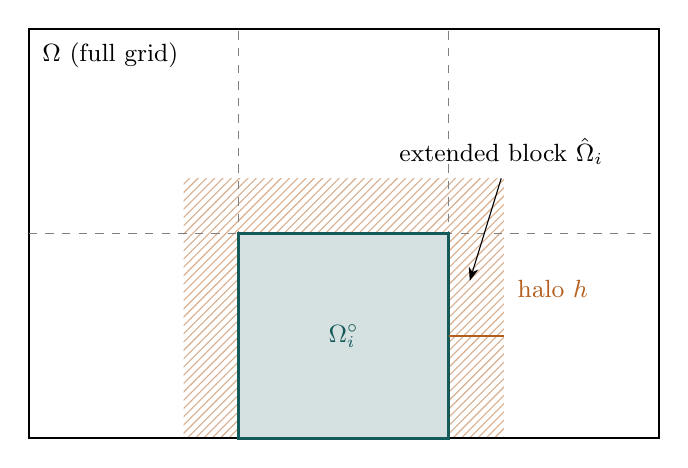
\begin{tikzpicture}[scale=1.0]
  % full domain
  \draw[thick] (0,0) rectangle (8,5.2);
  \node[anchor=north west] at (0.05,5.15) {\small $\Omega$ (full grid)};
  % interior partition lines (3x2 interior blocks)
  \foreach \x in {2.6667,5.3333} {\draw[gray,dashed] (\x,0) -- (\x,5.2);}
  \foreach \y in {2.6} {\draw[gray,dashed] (0,\y) -- (8,\y);}
  % extended (halo) block behind, for center-bottom patch
  \begin{scope}[on background layer]
    \fill[pattern=north east lines, pattern color=accent2!50]
      (2.6667-0.7,0) rectangle (5.3333+0.7,2.6+0.7);
  \end{scope}
  % interior block highlighted
  \fill[accent!18] (2.6667,0) rectangle (5.3333,2.6);
  \draw[accent,very thick] (2.6667,0) rectangle (5.3333,2.6);
  \node[accent,font=\small\bfseries] at (4,1.3) {$\Omega_i^\circ$};
  % halo annotation
  \draw[accent2,thick] (5.3333,1.3) -- (5.3333+0.7,1.3);
  \node[accent2,font=\small,anchor=west] at (5.3333+0.75,1.9) {halo $h$};
  % overlap annotation (between interior block and right neighbor extended region)
  \node[font=\small,anchor=south] at (6.0,2.6+0.75) {extended block $\hat\Omega_i$};
  \draw[->,>=Stealth] (6.0,2.6+0.7) -- (5.6,2.0);
\end{tikzpicture}
\caption{Overlapping decomposition. Each subdomain predicts its interior block
$\Omega_i^\circ$ (teal) but reads inputs from the larger extended block
$\hat\Omega_i$ (hatched), which includes a halo of width $h$ drawn from
neighboring cells. Interior blocks tile the domain; extended blocks overlap.}
\label{fig:decomp}
\end{figure}

\begin{figure}[t]
\centering
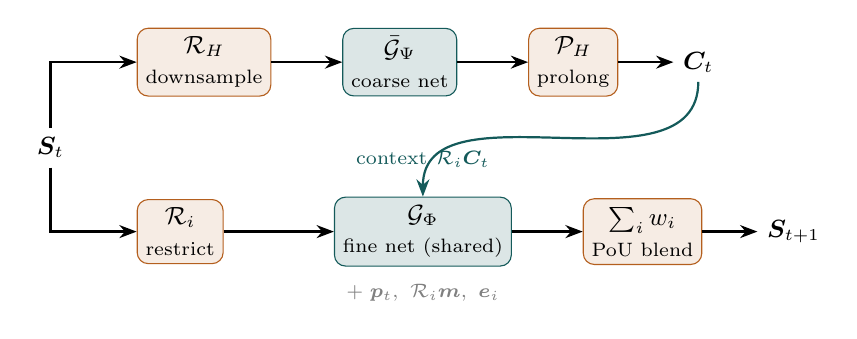
\begin{tikzpicture}[
  node distance=6mm and 9mm,
  box/.style={draw,rounded corners,align=center,minimum height=8mm,inner sep=3pt,font=\small,fill=boxbg},
  net/.style={box,fill=accent!15,draw=accent},
  op/.style={box,fill=accent2!12,draw=accent2},
  io/.style={align=center,font=\small\bfseries},
  ar/.style={-{Stealth[length=2.2mm]},thick},
]
  \node[io] (S) {$\bm S_t$};
  % coarse path (top)
  \node[op,above right=4mm and 8mm of S] (DH) {$\Rop_H$\\\scriptsize downsample};
  \node[net,right=of DH] (GC) {$\Gcoarse$\\\scriptsize coarse net};
  \node[op,right=of GC] (PH) {$\mathcal P_H$\\\scriptsize prolong};
  \node[io,right=7mm of PH] (C) {$\bm C_t$};
  % fine path (bottom)
  \node[op,below right=4mm and 8mm of S] (Ri) {$\Rop_i$\\\scriptsize restrict};
  \node[net,right=14mm of Ri] (GF) {$\Gfine$\\\scriptsize fine net (shared)};
  \node[op,right=of GF] (BL) {$\sum_i w_i$\\\scriptsize PoU blend};
  \node[io,right=7mm of BL] (Snext) {$\bm S_{t+1}$};
  % arrows
  \draw[ar] (S) |- (DH);
  \draw[ar] (DH) -- (GC);
  \draw[ar] (GC) -- (PH);
  \draw[ar] (PH) -- (C);
  \draw[ar] (S) |- (Ri);
  \draw[ar] (Ri) -- (GF);
  \draw[ar] (GF) -- (BL);
  \draw[ar] (BL) -- (Snext);
  % context injection into fine net
  \draw[ar,accent] (C) to[out=-90,in=90] (GF.north);
  \node[font=\scriptsize,accent,anchor=south] at ($(GF.north)+(0.0,0.25)$) {context $\Rop_i\bm C_t$};
  % params + geometry note
  \node[font=\scriptsize,gray,anchor=north] at ($(GF.south)+(0,-0.1)$) {$+\;\bm p_t,\ \Rop_i\bm m,\ \bm e_i$};
\end{tikzpicture}
\caption{One step of the two-level update. Top: a cheap coarse predictor produces
a low-resolution global next state, prolonged to the fine grid as a context field
$\bm C_t$. Bottom: a shared fine network predicts each patch from its restricted
state, halo, geometry, parameters, positional encoding $\bm e_i$, and the coarse
context. Patch predictions are blended by the partition of unity into
$\bm S_{t+1}$.}
\label{fig:dataflow}
\end{figure}

\subsection{Coarse global level}
Let $\Rop_H$ average-pool the fine state by an integer factor $r$ onto a coarse
grid of shape $(N_z/r)\times(N_y/r)\times(N_x/r)$, and let $\mathcal P_H$ be the
matching (trilinear) prolongation back to the fine grid. A coarse one-step
network $\Gcoarse$ predicts the coarse next state, and its prolongation is the
context field:
\begin{align}
\bar{\bm S}_t &= \Rop_H \bm S_t, &
\bar{\bm S}_{t+1} &= \Gcoarse\!\left(\bar{\bm S}_t,\ \bm p_t,\ \Rop_H \bm m\right), &
\bm C_t &= \mathcal P_H \bar{\bm S}_{t+1}.
\label{eq:coarse}
\end{align}
Because the coarse grid is small (a factor $r^3$ fewer cells), this pass is
cheap. Since the surrogate is translation-equivariant and resolution-flexible,
$\Gcoarse$ can reuse the fine weights ($\Psi=\Phi$, one network applied at two
resolutions) or be a smaller dedicated network; reusing weights is the leaner
default and is the recommended starting point.

\subsection{Fine-scale local update}
Each patch receives its restricted state, geometry, the restricted coarse
context, and a positional/boundary encoding $\bm e_i$ (e.g.\ signed distance to
the global boundary, so an edge patch can behave differently from an interior
one). The network predicts a \emph{residual} (delta-state) rather than the next
state directly, which is the standard choice for stable time-steppers:
\begin{align}
\hat{\bm x}_i &= \big[\, \Rop_i \bm S_t \,\|\, \Rop_i \bm m \,\|\, \Rop_i \bm C_t \,\|\, \bm e_i \,\big],
& \text{(channel-wise concatenation)} \\
\Delta_i &= \Gfine(\hat{\bm x}_i,\ \bm p_t),
& \hat{\bm S}_i = \big(\Rop_i \bm S_t + \Delta_i\big)\big|_{\Omega_i^\circ}.
\label{eq:fine}
\end{align}
The prediction is computed on the extended block and then cropped to the interior
$\Omega_i^\circ$: the halo cells are needed as input context but their outputs,
which lack their own neighbors, are discarded.

\subsection{Partition-of-unity merge}
The global next state is the windowed sum of the interior predictions:
\begin{equation}
\boxed{\;\bm S_{t+1} \;=\; \sum_{i=1}^{M} \Eop_i\!\big(\, w_i \odot \hat{\bm S}_i \,\big)\;}
\label{eq:merge}
\end{equation}
where $\odot$ is point-wise multiplication broadcast over channels. Property
\eqref{eq:pou} guarantees that, in any region where patches overlap, the
prediction is a convex combination of the patches that cover it; away from
overlaps a single window equals $1$ and the patch is used directly. Smooth
windows suppress the seams that abrupt cropping would leave
\cite{ronneberger2015unet,bartal2023multidiffusion}.

\begin{figure}[t]
\centering
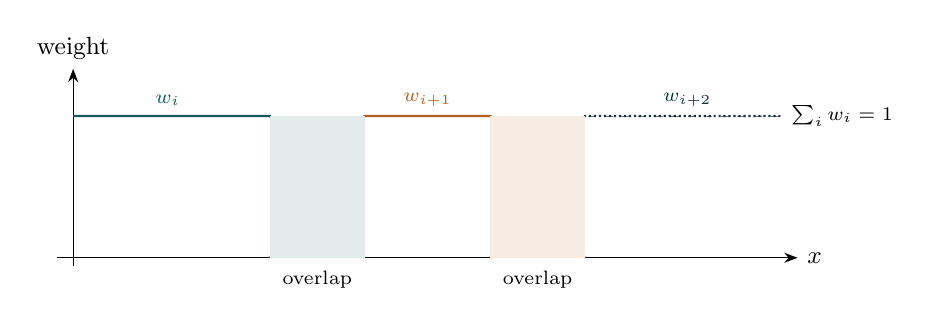
\begin{tikzpicture}[scale=1.0]
  \def\H{1.8}
  % axes
  \draw[->,>=Stealth] (-0.2,0) -- (9.2,0) node[right,font=\small] {$x$};
  \draw[->,>=Stealth] (0,-0.1) -- (0,2.4) node[above,font=\small] {weight};
  \draw[dashed,gray] (0,\H) -- (9,\H) node[right,font=\scriptsize,black] {$\sum_i w_i = 1$};
  % three trapezoidal windows, overlapping
  \draw[accent,thick] (0,\H) -- (2.5,\H) -- (3.7,0);                       % w1
  \draw[accent2,thick] (2.5,0) -- (3.7,\H) -- (5.3,\H) -- (6.5,0);          % w2
  \draw[accent!60!black,thick,densely dotted] (5.3,0) -- (6.5,\H) -- (9,\H);% w3
  % overlap shading
  \fill[accent!12] (2.5,0) rectangle (3.7,\H);
  \fill[accent2!12] (5.3,0) rectangle (6.5,\H);
  \node[font=\scriptsize,accent] at (1.2,\H+0.2) {$w_i$};
  \node[font=\scriptsize,accent2] at (4.5,\H+0.2) {$w_{i+1}$};
  \node[font=\scriptsize,accent!60!black] at (7.8,\H+0.2) {$w_{i+2}$};
  \node[font=\scriptsize,anchor=north] at (3.1,-0.05) {overlap};
  \node[font=\scriptsize,anchor=north] at (5.9,-0.05) {overlap};
\end{tikzpicture}
\caption{Partition-of-unity windows along one axis. Inside the overlap regions
two windows ramp so their sum stays $1$; the merge \eqref{eq:merge} is therefore
a smooth blend across patch boundaries.}
\label{fig:pou}
\end{figure}

\subsection{Optional divergence projection}
If residual velocity divergence at patch seams remains a problem after the coarse
level is added, an inexpensive Helmholtz projection restores
$\nabla\!\cdot\!\bm u = 0$. Solve a pressure-like Poisson problem and correct the
velocity,
\begin{equation}
\nabla^2 \phi = \nabla\!\cdot\!\bm u^{\star}, \qquad
\bm u \leftarrow \bm u^{\star} - \nabla \phi,
\label{eq:proj}
\end{equation}
where $\bm u^{\star}$ is the blended velocity from \eqref{eq:merge}. On the
coarse grid this solve is cheap and can use an FFT (periodic directions) or a few
multigrid sweeps; applying it at the coarse level and prolonging the correction
keeps cost negligible. Treat \eqref{eq:proj} as an optional, physics-based
safeguard, not a default.

\subsection{Inference}
Algorithm~\ref{alg:rollout} is the full autoregressive rollout. The halo for each
patch is read directly from the current global field, so neighbor information at
step $t$ is exactly the merged state from step $t-1$ --- no separate boundary
buffer is needed.

\begin{algorithm}[t]
\caption{Two-level domain-decomposed rollout (inference)}
\label{alg:rollout}
\begin{lstlisting}[style=pseudo]
Input: initial state S0, params {p_t}, geometry m, steps T
Input: fine net G, coarse net Gbar, operators R_H, P_H, R_i, E_i, windows w_i
S <- S0
for t = 0 to T-1 do
    # ---- coarse global context (Eq. 4) ----
    Sbar     <- Restrict R_H (S)                 # average-pool by factor r
    Sbar_next<- Gbar(Sbar, p_t, R_H(m))          # cheap low-res step
    C        <- Prolong P_H (Sbar_next)          # context on fine grid
    # ---- fine patches, embarrassingly parallel (Eq. 5) ----
    for each subdomain i do
        x_i   <- concat( R_i(S), R_i(m), R_i(C), e_i )
        dS_i  <- Predict G(x_i, p_t)             # residual on extended block
        Shat_i<- crop_to_interior( R_i(S) + dS_i )
    end for
    # ---- partition-of-unity merge (Eq. 6) ----
    S <- Blend  sum_i E_i( w_i * Shat_i )
    # ---- optional divergence projection (Eq. 7) ----
    if enforce_divergence_free then S <- Project(S)
    emit S as state at time t+1
end for
return trajectory {S_1, ..., S_T}
\end{lstlisting}
\end{algorithm}

\subsection{Training objective}
Train on patches cropped from full-domain reference simulations so the network
sees realistic halos. For a sampled time $t$ and patch $i$, with delta target
$\bm d_i = \Rop_i^\circ \bm S_{t+1}^{\text{ref}} - \Rop_i^\circ \bm S_t$ on the
interior, the loss combines four terms:
\begin{equation}
\mathcal L \;=\;
\underbrace{\big\| \Delta_i|_{\Omega_i^\circ} - \bm d_i \big\|^2}_{\text{one-step}}
\;+\; \lambda_{\mathrm{pf}}\,\mathcal L_{\mathrm{pf}}
\;+\; \lambda_{\mathrm{if}} \!\!\sum_{j\in\mathcal N(i)}\!\! \big\| \hat{\bm S}_i - \hat{\bm S}_j \big\|^2_{\Omega_i\cap\Omega_j}
\;+\; \lambda_{\mathrm{div}}\, \big\| \nabla\!\cdot\!\hat{\bm u}_i \big\|^2 .
\label{eq:loss}
\end{equation}
The \emph{interface} term penalizes disagreement between neighboring patches on
their overlap, directly training seam consistency; the \emph{divergence} term is
a soft physics constraint that complements the coarse level on the elliptic
coupling. The \emph{pushforward} term $\mathcal L_{\mathrm{pf}}$ is the existing
trick \cite{brandstetter2022mppde}: unroll $K$ steps through the full merge
(Algorithm~\ref{alg:rollout}) under \texttt{no\_grad}, then take one
gradient-tracked step against the snapshot at $t+K$, so the network is trained on
its own (merged) predictions. A coarse-level term
$\|\bar{\bm S}_{t+1}-\Rop_H\bm S_{t+1}^{\text{ref}}\|^2$ supervises $\Gcoarse$.
Algorithm~\ref{alg:train} sketches one optimizer step.

\begin{algorithm}[t]
\caption{One training step (patch-based, with pushforward and interface terms)}
\label{alg:train}
\begin{lstlisting}[style=pseudo]
Require: reference trajectories; pushforward depth K; weights lambda_*
sample a trajectory and a start time t; sample a tile group {i} and neighbors N(i)
S <- S_t^ref
# pushforward warm-up: K-1 merged steps without gradients
with no_grad:
    for k = 1 to K-1 do  S <- one_step(S, p_{t+k-1})   # Algorithm 1 body
# one gradient-tracked step
C        <- Prolong P_H ( Gbar(Restrict R_H(S), p_{t+K-1}, R_H(m)) )
for each i do
    dS_i   <- G( concat(R_i(S),R_i(m),R_i(C),e_i), p_{t+K-1} )
    Shat_i <- crop_to_interior( R_i(S) + dS_i )
end for
L  <- onestep(dS, d) + lambda_if * interface(Shat, N)
      + lambda_div * divergence(Shat) + lambda_c * coarse(Sbar_next, S_{t+K}^ref)
backprop L; optimizer.step()
\end{lstlisting}
\end{algorithm}

\subsection{Defaults and hyperparameters}
Table~\ref{tab:hyper} lists sensible starting values; the two that most affect
quality are the halo width (set from the receptive field) and the coarsening
factor.

\begin{table}[t]
\centering\small
\begin{tabularx}{\textwidth}{@{}l l Y@{}}
\toprule
\textbf{Symbol} & \textbf{Default} & \textbf{Guidance} \\
\midrule
Interior block $n$ & $32$--$64$ & Largest that trains comfortably in memory at depth. \\
Halo width $h$ & $h \ge \rho$ & At least the effective receptive-field radius $\rho$; estimate $\rho$ empirically \cite{ye2024lno}, and keep $h$ above the urban canopy length scale. \\
Overlap / taper $\delta$ & $h$ & Hann taper over the overlap band; wider $\delta$ = smoother seams, more redundancy. \\
Coarsening $r$ & $4$--$8$ & Coarse grid resolves the large-scale/pressure field; smaller $r$ if global coupling dominates. \\
Pushforward $K$ & $2$--$4$ & As in the existing trainer; raise if rollout drifts. \\
$\lambda_{\mathrm{if}},\lambda_{\mathrm{div}},\lambda_{\mathrm c}$ & $0.1,\,0.01,\,1$ & Start interface and divergence small; tune on a held-out rollout. \\
\bottomrule
\end{tabularx}
\caption{Recommended starting hyperparameters for Recommendation~A.}
\label{tab:hyper}
\end{table}

\section{Recommendation B --- consistent halo exchange (exact tiling)}\label{sec:recB}

Recommendation~B trades the coarse level and blending for a guarantee: with a
known receptive field and halo exchange, the tiled rollout reproduces a
whole-domain rollout exactly, with no seams. It is the better choice if blended
overlaps in~A leave visible artifacts, or if exact reproducibility against a
reference is required.

\subsection{Exactness condition}
Suppose the network's output at an interior cell depends only on inputs within a
radius $\rho$ (its receptive field). If the halo satisfies $h\ge\rho$, then every
interior cell of $\Omega_i^\circ$ sees exactly the same inputs it would have seen
in a whole-domain evaluation. Hence
\begin{equation}
\big(\Gfine(\bm S_t)\big)\big|_{\Omega_i^\circ}
= \big(\Rop_i^\circ \Gfine(\Rop_i \bm S_t)\big),
\qquad\text{so}\qquad
\bigsqcup_{i} \Rop_i^\circ \Gfine(\Rop_i \bm S_t) = \Gfine(\bm S_t),
\label{eq:exact}
\end{equation}
where $\bigsqcup$ is the disjoint tiling of interiors (no overlap, no blend). The
prediction is identical to the untiled network; the only requirement is that
halos are refilled from neighbors at \emph{every} step, since the receptive field
grows by $\rho$ per step \cite{barwey2024consistentgnn,ronneberger2015unet}.

\subsection{Optional per-step Schwarz iteration for global coupling}
Equation~\eqref{eq:exact} reproduces the network, but the network itself is still
local, so it inherits the same elliptic-coupling limitation. To recover global
coupling without a coarse level, wrap the patch update in a Schwarz iteration:
exchange halos and re-predict a few times before accepting the step, so
information propagates several patch-widths per time step
\cite{li2020deepddm,huang2025operatorddm}. Algorithm~\ref{alg:schwarz} shows the
inner loop.

\begin{algorithm}[t]
\caption{Per-step consistent update with optional Schwarz sweeps}
\label{alg:schwarz}
\begin{lstlisting}[style=pseudo]
Input: state S at time t; sweeps n_s (n_s = 1 recovers the one-shot exact tiling)
S_work <- S
for s = 1 to n_s do
    for each subdomain i do                      # parallel
        S_work <- Exchange halos from neighbors      # refill ghost cells
        x_i    <- concat( R_i(S_work), R_i(m), e_i )
        Shat_i <- crop_to_interior( G(x_i, p_t) )
    end for
    S_work <- assemble disjoint interiors  (Eq. 8)
end for
return S_work                                    # = S_{t+1}
\end{lstlisting}
\end{algorithm}

\subsection{Trade-offs}
B's strengths are no seam blur and a clean equivalence to the untiled model; its
costs are that the receptive field must be known and bounded (normalization and
global-pooling layers break locality and must be avoided
\cite{buglakova2025tiling}), halo bookkeeping is more involved, and the Schwarz
sweeps add per-step cost. In practice B is attractive once a single-level local
model has been validated and the only remaining issue is seam exactness; A is the
better first build because the coarse level addresses the physics gap that B
papers over.

\section{Choosing between A and B}\label{sec:choice}

\begin{table}[h]
\centering\small
\begin{tabularx}{\textwidth}{@{}l Y Y@{}}
\toprule
 & \textbf{A --- two-level + blend} & \textbf{B --- consistent exchange} \\
\midrule
Global coupling & coarse network (built in) & only via Schwarz sweeps \\
Seams & smoothed by PoU window & none (exact), if $h\ge\rho$ \\
Extra cost / step & one cheap coarse pass & $n_s$ halo exchanges \\
Architecture constraints & few & bounded receptive field; no global norm \\
Implementation effort & moderate & higher \\
Best when & elliptic coupling matters (urban LES) & exact reproduction needed \\
\bottomrule
\end{tabularx}
\caption{A and B differ mainly in how they handle global coupling and seams.}
\label{tab:choice}
\end{table}

\noindent
Recommended order: build the single-level local model first (stage~1 of the
survey), add halo forcing across the rollout, then adopt \textbf{A} by introducing
the coarse level. Keep \textbf{B} as the route to take if seam exactness, rather
than physics coupling, becomes the binding constraint. The two are compatible: a
two-level model can also use consistent halo exchange at the fine level.

\section{Mapping onto the \texttt{pyurbanair} codebase}\label{sec:mapping}

The design reuses the existing stack with localized additions.

\begin{itemize}
\item \textbf{Data (\texttt{TransitionDataset}).} Add a patch-sampling mode that
returns extended blocks $\Rop_i\bm S_t$ with halos, the interior delta target
$\bm d_i$, the restricted geometry, and (for the interface term) the indices of
neighboring patches. The existing lazy NetCDF reads extend naturally to cropping
a sub-box per item.
\item \textbf{Architecture.} No change to the core 3D UNet/ConvNeXt is required:
widen the stem to accept the extra context and positional channels
($\Rop_i\bm C_t$, $\bm e_i$), and switch the head to predict a residual
$\Delta_i$. Replace any batch-dependent normalization with a patch-independent
variant to avoid seam artifacts \cite{buglakova2025tiling}.
\item \textbf{Coarse level.} Reuse the same network at coarse resolution (it is
already resolution-flexible via the pad-to-multiple logic), or register a small
dedicated coarse preset under
\texttt{conf/neural\_surrogate\_architectures/}.
\item \textbf{Rollout / forward model.}
\texttt{NeuralSurrogateForwardModel.run\_single} currently advances the whole
grid; wrap it with the loop of Algorithm~\ref{alg:rollout} (coarse step, parallel
patch predictions, PoU merge). The domain check that today rejects a grid
mismatch is relaxed: the trained \emph{patch} size is the invariant, and the
\emph{global} grid becomes a free parameter --- which is the entire point of the
decomposition.
\item \textbf{Training.} The generic \texttt{Trainer} already supports the
pushforward unroll; extend its loss to include the interface, divergence, and
coarse terms of \eqref{eq:loss}, computed over the sampled tile group.
\end{itemize}

\noindent
A reasonable first milestone is stage~1 plus the coarse level on a single
moderate case where a whole-domain surrogate still fits, so the tiled two-level
prediction can be validated directly against both the LES reference and the
untiled surrogate before scaling the global grid.

\bibliographystyle{plain}
\bibliography{references}

\end{document}
